\chapter{An evaluation on the utility of the fingerprinting schemes}\label{chapter:Utility}


\section{Quality effects on fingerprinted datasets}\label{sec:quality}
To get an insight into how the fingerprinting scheme affects the quality of the data that is disturbed by perturbations, we calculate the mean and variance of the values of an attribute. 
In this section, we first present the analysis and the empirical evaluation of changes in these two measures for each of the fingerprinting schemes described in \Cref{sec:Fingerprinting}. 
Exclusively, for the fingerprinting scheme for categorical data, we use a different quality measurement since the mean and variance do not apply to the categorical values. 
Instead, we count the number of changes in the data introduced by fingerprinting. 

\subsection{AK Scheme}
The procedure of embedding the fingerprint is determined by the owner's secret key $\mathcal{K}$, primary key attribute \textit{P} and controlled by parameters $\gamma$, \textit{v} and $\xi$.
In a dataset with $\eta$ tuples, on average $\eta/\gamma$ tuples are selected for marking. 
In a selected tuple a single bit of a single attribute will be selected for marking. 
Mark value is calculated as a result of applying XOR function on fingerprint bit and pseudorandomly selected mask bit.
The mark bit value will half of the times match the original value, on average, and therefore leave the selected bit unchanged.
Considering that the probability of selecting a value for marking is $1/(\gamma v)$, i.e. one over the number of selected tuples times number of attributes, and the probability that the mark bit differs from the original bit value is $1/2$, we obtain the probability that the value will be selected and changed

\begin{equation}
    P\{L_i=1\} = 1 - P\{L_i=0\} = \frac{1}{2\gamma v}
\end{equation}

where $L_i$ equals 1 if the value of a certain attribute of tuple \textit{i} is selected and changed (in contrast, it equals 0 if the new value doesn't differ from the original value).

In addition, we assume that the original values of an attribute in the dataset are $x_1,x_2,...,x_{\eta}$ and the values of the attribute after fingerprinting are $x_1+\Delta_1,x_2+\Delta_2,...,x_{\eta}+\Delta_{\eta}$. 
\{$\Delta_1,\Delta_2,...,\Delta_\eta$\} represent the error caused by fingerprinting.
They are independent and identically distributed random variables. 
We further assume the representation of $\Delta_i, 1 \leq i \leq \eta$, 

\begin{equation}
\Delta_i = L_i S_i 2^{U_i}
\end{equation}

where $S_i \in \{-1,1\}$ depending on whether the perturbed value is smaller or greater than the original, both with probability 0.5, and $U_i \in \{0,1,...,\xi-1\}$ is uniformly distributed variable representing position of the marked bit. 
\paragraph{Mean}
The mean value of the original attribute values is

\begin{equation}
\overline{x}=(1/\eta)\sum_{i=1}^{\eta}x_i
\end{equation}

and the mean of the attribute values after embedding the fingerprint is

\begin{equation}
\overline{x}'=\overline{x}+\overline{\Delta}
\end{equation} 

where

\begin{equation}
\overline{\Delta}=(1/\eta)\sum_{i=1}^{\eta} \Delta_i
\end{equation}

The expected error of a single attribute value is

\begin{equation}
E[\Delta_i]=\frac{1}{2} L_i 2^{U_i} - \frac{1}{2} L_i 2^{U_i} = 0, \forall i:1 \leq i \leq \eta
\end{equation}

thus the expected error in attribute mean value after embedding the fingerprint is 

\begin{equation}
E[\overline{\Delta}]=0
\end{equation}

\paragraph{Variance}
The variance of the original attribute values is given by 

\begin{equation}
V_x=\frac{1}{\eta}\sum_{i=1}^{\eta} (x_i - \overline{x})^2
\end{equation}

and the variance of the perturbed attribute values after the fingerprint insertion is 

\begin{equation}
V_{x+\Delta}=\frac{1}{\eta}\sum_{i=1}^{\eta}[(x_i+\Delta_i)-(\overline{x}+\overline{\Delta})]^2
\end{equation}

After applying some algebra, the error in variance is given by

\begin{equation}
V_{x+\Delta}-V_x = \frac{1}{\eta} \sum_{i=1}^{\eta}(\Delta_i-\overline{\Delta})^2 + 2\cdot\frac{1}{\eta}\sum_{i=1}^{\eta}(x_i-\overline{x})(\Delta_i-\overline{\Delta})
\end{equation}

The expected error in computing the variance is given by

\begin{equation}
E[V_\Delta]\approx\frac{2^{2\xi}}{6\gamma v \xi}
\end{equation}


\begin{table}[ht]
\centering
\caption{Change in variance introduced by fingerprinting with AK Scheme}
\label{table:AK-mean-var}
\resizebox{\textwidth}{!}{
\begin{tabular}{|lrr|rr|rr|rr|rr|} 
 \hline
 & & $\gamma$ & \multicolumn{2}{c|}{100} & \multicolumn{2}{c|}{50} & \multicolumn{2}{c|}{25} & \multicolumn{2}{c|}{12} \\ 
 & & $\xi$ & \multicolumn{1}{c}{4}&\multicolumn{1}{c|}{8}&\multicolumn{1}{c}{4}&\multicolumn{1}{c|}{8}&\multicolumn{1}{c}{4}&\multicolumn{1}{c|}{8}&\multicolumn{1}{c}{4}&\multicolumn{1}{c|}{8}\\
 \hline
 & \multicolumn{2}{c|}{Expected error in variance} & 0 & 1.4 & 0.01 & 2.7 & 0.02 & 5.5 & 0.04 & 11.4 \\
 \hline
 \textbf{Attribute} & \textbf{Mean} & \textbf{Variance} & & & & & & & & \\
 \hline
 Elevation & 2,959 & 78,391 & 0 &+1& 0 &+1&+1&+5&+1& +9 \\
 \hline
 Aspect & 156 & 12,525 &0 &+1&0 &+1&+1&+5& 0 & +8 \\
 \hline
 Slope & 14 & 56 & 0 &+1 &0 & +3&0 & +5&0  & +11 \\
 \hline
 HD-Hydrology & 269 & 45,177 &0 & +1& 0 &+1 &0 &+2 &+1  &+2  \\
 \hline
 VD-Hydrology & 46 & 3,398 & 0 & +1 & 0 & +2 &0 &+4 &0  &+9  \\
 \hline
 HD-Roadways & 2,350 & 2,431,276 & 0 & +10 & 0 & +10 & \textcolor{red}{-1} & +5 & +2  & +37  \\
 \hline
 Hillshade-9am & 212 & 717 & 0&+1 &0 &+2 &0 &+4 &  0 &+9  \\
 \hline
 Hillshade-noon & 223 & 391 & 0& +1&0 &+2 &0 &+4 &0  & +10 \\
 \hline
 Hillshade-3pm & 143 & 1,465 & 0& +1& 0&+2 &0 &+4 &0  &+8  \\
 \hline
 HD-Fire-Points & 1,980 & 1,753,493 & 0 & \textcolor{red}{-2} & 0 & +5 & 0 & +8 & +1 & +30  \\
 \hline
\end{tabular}
}
\end{table}

\paragraph{Experiments}
Experimental results are obtained by embedding a fingerprint into the Forest dataset. 
We choose the set of following values for parameter $\gamma$ = \{12,25,50,100\}, and $\xi$ = \{4,8\}. 
Table \ref{table:AK-mean-var} contains recorded changes in the variance introduced by fingerprinting for each of the attributes and parameter setting.
The results support the analysis previously made on errors in the mean and variance of the attribute values.
The error in the mean in all of the cases of this experiment was $<0.01$, so only the error in the variance is presented.
The largest changes are expectedly occurring when $\gamma$ is small and $\xi$ is big, i.e. when more tuples are selected and more bits of the value are available for marking. 
The errors in variance between cases with the same $\gamma$ value and different $\xi$ differ significantly, implying that imperceptibility of the fingerprint is highly sensitive to the number of LSBs available for marking.
Original values of the variances, in general, do not affect the relative error of perturbed values.  
In rare cases, the introduced errors result in a decrease of the variance, however, the change is in the same range as in cases where the variance increases. 


\subsection{Block Scheme}

Experimental results are obtained by embedding a fingerprint into the Forest dataset. 
We choose the set of following values for parameter $\beta$ = \{30,25,15,10\}, and $\xi$ = \{4,8\}. 
Table \Cref{table:block-mean} contains recorded changes in mean introduced by fingerprinting for each of the attributes and parameter setting, and \Cref{table:block-var} changes in variance.
\begin{table}[h]
\centering
\caption{Change in mean introduced by fingerprinting with the Block Scheme}
\label{table:block-mean}
\begin{tabular}{|l r|c c| c c| c c| c c|} 
 \hline
 & $\beta$ & \multicolumn{2}{c|}{30} & \multicolumn{2}{c|}{25} & \multicolumn{2}{c|}{15} & \multicolumn{2}{c|}{10} \\ 
 & $\xi$ &4&8&4&8&4&8&4&8\\
 \textbf{Attribute} & \textbf{Mean} & & & & & & & & \\
 \hline
 Elevation & 2959 &  &  &  &  &  &  &  & \\
 \hline
 Aspect & 156 &  &  &  &  &  &  &  & \\
 \hline
 Slope & 14 &  &  &  &  &  & +1 &  & \\
 \hline
 HD-Hydrology & 269 &  &  &  &  &  &  &  & \\
 \hline
 VD-Hydrology & 46 &  &  &  & +1 &  & +1 &  & +1\\
 \hline
 HD-Roadways & 2350 &  &  &  &  &  &  &  & \\
 \hline
 Hillshade-9am & 212 &  &  &  &  &  &  &  & \\
 \hline
 Hillshade-noon & 223 &  &  &  &  &  &  &  & \textcolor{red}{-2}\\
 \hline
 Hillshade-3pm & 143 &  &  &  & \textcolor{red}{-1} &  & \textcolor{red}{-1} &  & \textcolor{red}{-1}\\
 \hline
 HD-Fire-Points & 1980 &  &  &  &  &  &  &  & \\
 \hline
\end{tabular}
\end{table}

\begin{table}[ht]
\centering
\caption{Change in variance introduced by fingerprinting with the Block Scheme}
\label{table:block-var}
\begin{tabular}{|l r|r r|r r|r r|r r|} 
 \hline
 & $\beta$ & \multicolumn{2}{c|}{30} & \multicolumn{2}{c|}{25} & \multicolumn{2}{c|}{15} & \multicolumn{2}{c|}{10} \\ 
 & $\xi$ & \multicolumn{1}{c}{4}&\multicolumn{1}{c|}{8}&\multicolumn{1}{c}{4}&\multicolumn{1}{c|}{8}&\multicolumn{1}{c}{4}&\multicolumn{1}{c|}{8}&\multicolumn{1}{c}{4}&\multicolumn{1}{c|}{8}\\
 \textbf{Attribute} & \textbf{Variance} & & & & & & & & \\
 \hline
 Elevation & 78391 & 0 & +13 & +1 & +15 & +1 & +48 & +1 & +178 \\
 \hline
 Aspect & 12525 & 0 & +7 & 0 & +12 & 0 & +35 & 0 & +127 \\
 \hline
 Slope & 56 & 0 & +12 & 0 & +18 & 0 & +48 & 0 & 0 \\
 \hline
 HD-Hydrology & 45177 & 0 & +6 & +1 & +4 & +1 & +13 & +2 & 0 \\
 \hline
 VD-Hydrology & 3398 & 0 & +10 & 0 & +15 & 0 & +38 & 0 & +87 \\
 \hline
 HD-Roadways & 2431276 & 0 & +3 & 0 & +3 & 0 & +44 & \textcolor{red}{-2} & 0 \\
 \hline
 Hillshade-9am & 717 & 0 & +11 & 0 & +15 & 0 & +41 & 0 & +8 \\
 \hline
 Hillshade-noon & 391 & 0 & +11 & 0 & +16 & 0 & +45 & 0 & +200 \\
 \hline
 Hillshade-3pm & 1465 & 0 & 0 & 0 & +13 & 0 & +35 & 0 & +160 \\
 \hline
 HD-Fire-Points & 1753493 & 0 & 0 & 0 & \textcolor{red}{-4} & 0 & +54 & 0 & +68 \\
 \hline
\end{tabular}
\end{table}

The error is primarily controlled by parameter $\beta$. 
We have previously discussed the expected average number of changes which is described with \Cref{eq:block-changes}. 
$\beta$ in denominator suggests that for smaller $\beta$ there will be more errors in the data introduced by the fingerprint. 
We can see that a larger number of errors expectedly introduces larger errors in variance from the \Cref{table:block-var}.
The smallest error of variance appears for $\beta=30$ and increases for smaller $\beta$ values.

A large difference in the error of variance is noticeable between different values of $\xi$ which defines the number of LSBs available for fingerprinting.
We expect larger errors if more LSBs are available for fingerprinting - bits of more significance are being potentially changed, therefore creating bigger distortions (also assumed from \Cref{eq:block-changes}).
The experiment results in \Cref{table:two-level-mean-var} and \Cref{table:block-mean} confirm this claim. 
Setting $\xi=4$ will result in no or very small errors of variance and mean.
Note that $\xi=8$ may change a value in the dataset up to $\pm 2^7=\pm 128$. 
Considering that most of the values in Forest dataset are in the range of $2^7$, $\xi=8$ is a rather big value. 
For example, in the attribute \textit{Slope} where the mean value is 14 (see \Cref{table:block-mean}), this may cause quite a perceptible modification. 
For attributes with a range of larger values, e.g. \textit{Aspect} with mean 156 or \textit{HD-Roadways} with mean 2350, the error of $\leq \pm 128$ causes slightly less perceptible modifications in single values compared to \textit{Slope}, however the overall variance is certainly affected. 
We see in \Cref{table:block-mean} that error in the mean is introduced only for $\xi=8$ and for attributes with the small mean value.
We have set $\xi=8$ for experiments purely to show the clear distinction of the ways that different values of $\xi$ affect the quality of the data. 
In practice, $\xi$ is set according to the values in the dataset and generally to the smaller values. When $\xi$ is set appropriately, in these experiments $\xi=4$, different values of $\beta$ do not affect the errors in mean and variance too much.

\subsection{Two-level Fingerprinting Scheme}

The embedding process is controlled by $\gamma_1$, $\gamma_2$ and $\xi$.
Using \Cref{eq:total-gamma}, a dataset with $\eta$ tuples will have $ \frac{1}{\gamma}=\frac{1}{\gamma_1}+(1-\frac{1}{\gamma_1})*\frac{1}{\gamma_2}$ tuples selected for marking. Due to the pseudo-random nature of bit marking, the selected bit's original value will half of the times match the mark. 
Thus, the probability that the value will be selected and changed is
\begin{equation}
    P\{L_i=1\} = 1- P\{L_i=0\}=\frac{1}{2\gamma} = \frac{1}{2\gamma_1} +(1-\frac{1}{\gamma_1})*\frac{1}{2\gamma_2}
\end{equation}

where $L_i$ equals 1 if the value of a certain attribute of tuple \textit{i} is selected and changed (in contrast, it equals 0 if the new value doesn't differ from the original value).

The authors of the proposed scheme in their work \cite{guo2006fragile} present the quality effects by measuring mean and variance before and after embedding. 
They show the results from experiments run on a portion of Forest Cover data ($\eta=5,000$) and where fingerprinting is applied to a single attribute - \textit{Elevation}. 
Both mean and variance showed minor absolute alteration ($\approx0.01$) and lead to the conclusion that the scheme preserves the utility of the data. 

We show the empirical results on change in mean and variance in a scenario with entire Forest Cover Type data ($\eta=581,012$). 
For our experiments we consider all 10 numerical attributes for marking ($v=10$) and set parameters as follows: $\gamma_1=\gamma_2=\{10, 25, 50, 100\}$, $\eta=\{4, 8\}$ and $L=96$.

\begin{table}[ht]
\centering
\caption{Change in variance introduced by fingerprinting using the Two-level Fingerprinting Scheme}
\label{table:two-level-mean-var}
\resizebox{\textwidth}{!}{
\begin{tabular}{|lrr|rr|rr|rr|rr|} 
 \hline
 & & $\gamma_1=\gamma_2$ & \multicolumn{2}{c|}{100} & \multicolumn{2}{c|}{50} & \multicolumn{2}{c|}{25} & \multicolumn{2}{c|}{10} \\ 
 & & $\xi$ & \multicolumn{1}{c}{4}&\multicolumn{1}{c|}{8}&\multicolumn{1}{c}{4}&\multicolumn{1}{c|}{8}&\multicolumn{1}{c}{4}&\multicolumn{1}{c|}{8}&\multicolumn{1}{c}{4}&\multicolumn{1}{c|}{8}\\
 \textbf{Attribute} & \textbf{Mean} & \textbf{Variance} & & & & & & & & \\
 \hline
 Elevation & 2959 & 78391 &+1  & +3& +1& +4 & +1 & +4& +1 & +14\\
 \hline
 Aspect & 156 & 12525 &0 & +3 &0& +7& 0& +15&0 & +36\\
 \hline
 Slope & 14 & 56 &0 & +1 &0& +2&0& +4& 0 & +10\\
 \hline
 HD-Hydrology & 269 & 45177 &0&+3 &0& +5&+1& +7& +2 & +10\\
 \hline
 VD-Hydrology & 46 & 3398 & 0& +1&0& +1&0& +3& 0 & +6\\
 \hline
 HD-Roadways & 2350 & 2431276 & \textcolor{red}{-1}& +12&0& +27&0& +31& +1 & +61 \\
 \hline
 Hillshade-9am & 212 & 717 & 0 & 0 & 0& +1&0& +2&0 &+6\\
 \hline
 Hillshade-noon & 223 & 391 & 0& +4& 0& +9&0& +18& 0 & +43\\
 \hline
 Hillshade-3pm & 143 & 1465 &0 &+1 & 0& +3&0& +5&0 & +13\\
 \hline
 HD-Fire-Points & 1980 & 1753493 &+1 & 0 & +1& +12&0& +19& +1 & +34\\
 \hline
\end{tabular}}
\end{table}

The total mark ratio in the embedding process is around $1/\gamma_1 + 1/\gamma_2$. 
\Cref{table:two-level-mean-var} shows that the change in variance increases for larger number of marks, i.e. smaller $\gamma_1$ and $\gamma_2$. 
The change, however, depends on the number of LSBs available for marking $\xi$ as well. 
By choosing a smaller value, the change of variance can be almost completely avoided. The smaller $\xi$ value, however, decreases the robustness of the scheme which needs to be taken into account when choosing the value of this parameter. This is discussed in \Cref{sec:Robustness}.
The mean value of any attribute did not change more than $0.01$ in any of the experiments.
These changes are minuscule enough to hold the claim that the alteration for fingerprinting does not affect the usability of the data.


\subsection{Fingerprinting scheme for categorical data}
The fingerprinting scheme that deals with categorical data requires a different type of measure for data utility since mean and variance are not applicable in this case. One possible measure is the number of changes introduced by marking the data.

We fingerprint the categorical values of the Adult dataset using the fingerprinting scheme for categorical data. Furthermore, we fingerprint the numerical attributes using the AK Scheme. 
\Cref{table:categorical-ak-mean} shows the utility effects on the Adult dataset (which contains 30,162 tuples) introduced by the fingerprinting scheme for categorical data. 
The utility of numerical attributes is still measured by mean and variance, where the difference in the mean is negligible (it does not exceed 0.02 and is therefore excluded from the table). The change in variance introduced by errors for numerical attributes is also rather small, as it was the case with previously presented schemes. 
For each categorical attribute, we count how many changes in values are introduced by the fingerprint.
The Number of values that change in a single categorical attribute is approximately $30,162/(2\gamma v )$. 
For the presented set of parameters, the introduced total number of changes is $<4\%$ of the total number of tuples in the dataset. 
Due to the random nature of fingerprint insertion process, the distributions of attributes are not significantly affected.


\begin{table}[ht]
\centering
\caption{Change in variance and value-flips introduced by fingerprinting with the fingerprinting scheme for categorical data and the AK Scheme, on the Adult dataset}
\label{table:categorical-ak-mean}
\begin{tabular}{|l r|r r|r r|r r|r r|} 
 \hline
 & $\gamma$ & \multicolumn{2}{c|}{50} & \multicolumn{2}{c|}{25} & \multicolumn{2}{c|}{12} & \multicolumn{2}{c|}{6}
 \\ 
 & $\xi$ &2&4&2&4&2&4&2&4 \\

 \textbf{Attribute} & \textbf{Variance} & & & & & & & & \\
 \hline
 Age & 173 & 0 & 0 & 0 & 0 & 0 & 0 & 0 & +0.05 \\
 \hline
 Capital Gain & 54,853,968 & \textcolor{red}{-1} & \textcolor{red}{-3} & \textcolor{red}{-5} & \textcolor{red}{-11} & \textcolor{red}{-23} & \textcolor{red}{-56} & \textcolor{red}{-31} & \textcolor{red}{-67}\\
 \hline
 Capital Loss & 163,457 & 0 & \textcolor{red}{-1} & 0 & \textcolor{red}{-1} & \textcolor{red}{-1} & \textcolor{red}{-2} & \textcolor{red}{-2} & \textcolor{red}{-5} \\
 \hline
 Hours per Week & 144 & 0 & 0 & 0 & 0 & 0 & +0.2 & 0 & +0.3 \\
 \hline
  & & \multicolumn{8}{c|}{\textbf{Value Changes} }\\
\hline
 Workclass & & 26 & 19 & 45 & 45 & 81 & 90 & 165 & 165\\
 \hline
 Education && 26 & 18 & 49 &43 & 83 & 84 & 172 & 173\\
 \hline
 Marital Status && 24 & 24 & 46 & 44 & 101 & 87 & 207 & 189\\
 \hline
 Occupation && 23 & 20 & 44 & 47 & 75 & 73 & 148 & 135\\
 \hline
 Relationship && 22 & 22 & 29 & 41 & 81 & 89 & 175 & 189\\
 \hline
 Race && 19 & 20 & 47 & 51 & 87 & 91 & 160 & 174\\
 \hline
 Sex && 12 & 5 & 19 & 13 & 39 & 25 & 77 & 46\\
 \hline
 Native country && 19 & 21 & 45 & 30 & 94 & 78 & 173 & 164\\
 \hline
 \end{tabular}
 \end{table}


\section{Impact of fingerprinting on Machine Learning models}\label{sec:Learning}
In this section, we evaluate the utility of fingerprinted datasets by measuring the difference in the performance of classifiers for a predictive task, using the original and the fingerprinted dataset. 
We use \textit{accuracy} and \textit{F1} as performance measures. 
In Machine Learning, binary classification is the task of classifying the elements of a given set into two groups (also, categories or classes). 
Given a classification of a specific data set, there are four basic combinations of the actual data class and the assigned class: true positives (TP; actual positive and predicted positive), false positives (FP; actual negative and predicted positive), true negatives (TN; actual negative and predicted negative) and false negatives (FN; actual positive and predicted negative), where "positive" and "negative" represent two classes. 
These combinations can be arranged into a 2x2 contingency table as shown in \Cref{fig:confusion-matrix-binary}.

\begin{figure}
    \centering
    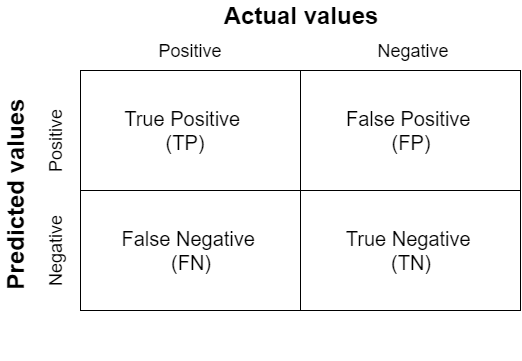
\includegraphics[width=0.6\textwidth]{Figures/confusion.png}
    \caption{Combinations of actual data classes and assigned classes in binary classification}
    \label{fig:confusion-matrix-binary}
\end{figure}

A calculation of the classification accuracy and F1 score is based on a number of occurrences of each combination in the classification. 
Accuracy is the ratio of a number of correct predictions to the total number of input samples.
Accuracy of a binary classification is defined as:
\begin{equation}\label{eq:accuracy-binary}
    accuracy = \frac{TP+TN}{P+N}
\end{equation}
where $P = TP+FP$ and $N = TN+FN$.
F1 score of binary classification is the harmonic average of the precision and the recall.
Precision, recall and F1 score for the binary classification are defined as follows:
\begin{equation}
    precision = \frac{TP}{TP+FP}
\end{equation}
\begin{equation}
    recall = \frac{TP}{TP+FN}
\end{equation}
\begin{equation}\label{eq:f1-binary}
    F1 = 2 \cdot \frac{precision \cdot recall}{precision + recall}
\end{equation}

The metrics are shown graphically in \Cref{fig:performance-metrics}.

\begin{figure}
    \centering
    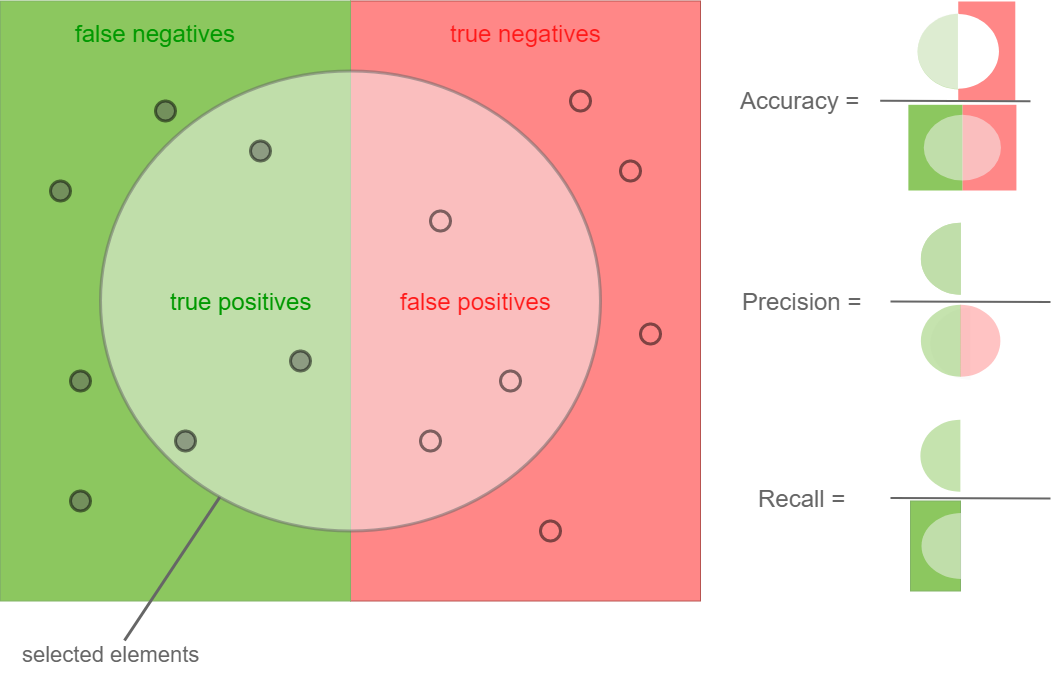
\includegraphics[width=0.8\textwidth]{Figures/metrics.png}
    \caption{Classification performance metrics}
    \label{fig:performance-metrics}
\end{figure}

Multiclass (or multinomial) classification is the task of classifying the elements of a given set into three or more groups (categories, classes). 
It can be denoted as a function $g(x)$ that on input $x$ returns one of the classes ${1,...,K}$.
Similarly to the binary classification, we can distinguish the combinations of actual data class and the predicted one. In this case, we have true positives, false positives and false negatives associated with each class $i$.
$\text{TP}_i$ denotes the instances from the class $i$ that are predicted to be in the class $i$, $\text{FP}_i$ are instances belonging to another class, falsely predicted to be in the class $i$, and $\text{FN}_i$ are the instances from the class $i$ falsely predicted to be in some other class. 

The accuracy of the multinomial classification is calculated as:
\begin{equation}\label{eq:accuracy-multiclass}
    accuracy = \frac{1}{\eta}\cdot \sum_{i=1}^{K}\text{TP}_i
\end{equation}
where $\eta$ is a total number of data instances. Note that \Cref{eq:accuracy-multiclass} is the general form that applies to the binary classification as well. 

For multiclass classification, precision and recall can be micro- or macro-averaged, therefore also can be F1 score.
The micro-averaged precision and recall are defined as follows:
\begin{equation}
    precision_{micro} = \frac{\sum_{i=1}^{K}\text{TP}_i}{\sum_{i=1}^{K}\text{TP}_i + \text{FP}_i}
\end{equation}
\begin{equation}
    recall_{micro} = \frac{\sum_{i=1}^{K}\text{TP}_i}{\sum_{i=1}^{K}\text{TP}_i + \text{FN}_i}
\end{equation}
Therefore, the micro F1 score is: 
\begin{equation}
    F1_{micro} = 2 \cdot \frac{precision_{micro} \cdot recall_{micro}}{precision_{micro} + recall_{micro}}
\end{equation}
If micro F1 is a large value, this indicates that a classifier performs well overall, however it is not sensitive to the performance of individual classes. 
The macro-averaged precision and recall are:
\begin{equation}
    precision_{macro} = \frac{1}{K}\sum_{i=1}^{K}\frac{\text{TP}_i}{\text{TP}_i + \text{FP}_i}
\end{equation}
\begin{equation}
    recall_{macro} = \frac{1}{K}\sum_{i=1}^{K}\frac{\text{TP}_i}{\text{TP}_i + \text{FN}_i}
\end{equation}
Hence, the macro F1 score is:
\begin{equation}\label{eq:f1-macro}
    F1_{macro} = 2 \cdot \frac{precision_{macro} \cdot recall_{macro}}{precision_{macro} + recall_{macro}}
\end{equation}
A large macro F1 suggests that the classifier performs well for each individual class. The macro-average is therefore more suitable for data with an imbalanced class distribution.
All of the above metrics reach their best value at 1 for the perfect classifier and worst at 0.

\paragraph{Experimental setup}
We used three datasets for the experiments - the Forest dataset, the Adult dataset and the Credit dataset. Therefore, three different classifications have been analysed. 
In the Forest dataset, the target attribute is \textit{covertype} with 7 values, thus we are solving the multiclass classification problem. 
The accuracy is calculated as in \Cref{eq:accuracy-multiclass}. Furthermore, we choose to use macro averages for calculating the F1 score (\Cref{eq:f1-macro}) to avoid the misleading nature of micro averages when the class distribution is imbalanced.

In the Adult dataset, we are predicting the binary attribute \textit{income}. In the German Credit dataset, we are as well predicting the binary target attribute that classifies the data instance as good or bad credit risk. The binary classification is being performed and analysed for these two datasets and accordingly, the classification accuracy and F1 are calculated as \Cref{eq:accuracy-binary} and \Cref{eq:f1-binary}.

For all of our experiments, we use 10-fold cross-validation to evaluate Machine Learning models.
$k$-fold cross-validation is a resampling procedure used in Machine Learning to estimate the skill of a Machine Learning model on unseen data.
It generally results in a less biased or less optimistic estimate of the model skill than other methods, such as a simple train/test split. 
The procedure starts by shuffling the dataset randomly and splitting it into $k$ groups. In our experiments $k=10$. 
Each unique group is taken as a hold out (test dataset) while the remaining $k-1$ groups are taken as a training dataset.
It fits a model on the training set and evaluates it on the test set, retaining the evaluation score for that group.
At the end, we summarise the skill of the model using the sample of model evaluation scores.
In the experiments, we record the average of these scores. 

Generally, the goal was not to build models with best predictions but to compare the effectiveness of the fingerprinted data compared to the original.
Therefore, there is no advanced parameter optimisation included nor we dive into more complicated feature selection for building models, as it would shift the focus from the main goal. 
Still, we wanted to achieve the model performance levels rather close to the benchmark solutions available from numerous online sources\footnote{\url{https://www.kaggle.com/wenruliu/adult-income-dataset/kernels}}\footnote{\url{https://www.kaggle.com/c/forest-cover-type-prediction/kernels}} (the chosen datasets and the correlated classification problems are well known in the Machine Learning community).
Therefore, it was important to find good hyperparameters for each of the classification tasks and each classifier.
One possible solution besides the pure manual tuning is a random search over hyperparameters.
We set up a grid of hyperparameter values and select a limited number of random combinations to train the model and score on validations data.
This way we choose the combination of parameters giving the best score for our model.

We use Randomized Search with 10 iterations from the Python scikit-learn package\footnote{\url{https://scikit-learn.org/stable/}} for tuning most important hyperparameters. 
Evaluation within the random search is done using 10-fold cross-validation and F1 score (macro F1 in case of a multiclass classification). 

Finally, for our experiments, we use the following classifiers, all implemented in the Python scikit-learn package:
\begin{itemize}
    \item Decision Tree
    \item k-NN (k Nearest Neighbours)
    \item Logistic regression
    \item Random Forest
    \item Gradient Boosting
\end{itemize}

The experimental process in the following sections has the following steps:
\begin{enumerate}
    \item Use random search to tune the hyperparameters of the Decision Tree, k-NN, Logistic Regression, Random Forest and Gradient Boosting classifiers. In some of the experiments, we use only the subset of the classifiers above. 
    \item Train the model with the original dataset and score the classification accuracy and F1
    \item For each fingerprinting parameter combination $(\gamma, \xi)$ train the model with the fingerprinted dataset and score the classification accuracy and F1. Set the hyperparameters according to step 1.  
    \item Record the differences in the performance measures
    \item Steps 3 and 4 are repeated 10 times to get the average values. In every experiment, we fingerprint the data with a random choice of buyer's id and secret key.
    
\end{enumerate}


% Forest dataset
\subsection{Forest Cover Type}
The first set of experiments is made using the biggest of the three datasets - Forest Cover Type. 
We use the AK Scheme for fingerprinting the numerical attributes of the dataset.
The target attribute is \textit{covertype} and all the others are used as an input for a prediction. 
We use the following classifiers and set the following hyperparameters:
    \begin{itemize}
        \item Decision Tree: $max\_depth=5$, $criterion=entropy$
        \item Logistic Regression: $C=100$
        \item Random Forest: $n\_estimators=100$
    \end{itemize}
    The other hyperparameters are set to default values from the scikit-learn implementations of the classifiers.

The average differences are shown in \Cref{tab:dt_forest_diff,tab:lr_forest_diff,tab:rf_forest_diff} for Decision Tree, Logistic Regression and Random Forest, respectively.

\begin{table}[ht]
    \centering
    \caption{Effects on F1 score and classification accuracy of a Decision Tree model trained with the Forest Cover Type dataset}
    \label{tab:dt_forest_diff}
    \resizebox{\textwidth}{!}{
    \begin{tabular}{|l|rr|rr|rr||rr|}
    \hline
        &  \multicolumn{2}{c|}{$\xi=2$} &  \multicolumn{2}{c|}{$\xi=4$} &  \multicolumn{2}{c||}{$\xi=6$} & 
        \multicolumn{2}{c|}{average} \\
        & F1 & acc. & F1 & acc.  & F1 & acc. & F1 & acc. \\
        \hline
         $\gamma=100$ & 0\% & 0\% & 0\% & \textcolor{red}{-0.01\%} & 0\% & \textcolor{red}{-0.01\%} & 0\% & \textcolor{red}{-0.01\%}\\
         \hline
         $\gamma=50$ & 0\% & \textcolor{red}{-0.02\%} & 0\% & 0\% & 0\% & +0.01\% & 0\% & 0\%\\
         \hline
         $\gamma=25$ & 0\% & \textcolor{red}{-0.02\%} & +0.02\% & +0.01\% & \textcolor{red}{-0.03\%} & \textcolor{red}{-0.01\%} & 0\% & \textcolor{red}{-0.01\%}\\
         \hline
         $\gamma=12$ & \textcolor{red}{-0.01\%} & \textcolor{red}{-0.02\%} & \textcolor{red}{-0.01\%} & 0\% & \textcolor{red}{-0.01\%} & \textcolor{red}{-0.10\%} & \textcolor{red}{-0.01\%} & \textcolor{red}{-0.04\%}\\
         \hline
         $\gamma=6$ & \textcolor{red}{-0.01\%} & 0\% & \textcolor{red}{-0.04\%} & \textcolor{red}{-0.01\%} & \textcolor{red}{-0.19\%} & \textcolor{red}{-0.11\%} & \textcolor{red}{-0.08\%} & \textcolor{red}{-0.04\%}\\
         \hline
         \hline
         average & 0\% & \textcolor{red}{-0.1\%} & \textcolor{red}{-0.01\%} & 0\% & \textcolor{red}{-0.05\%} & \textcolor{red}{-0.04\%} & \textbf{\textcolor{red}{-0.07\%}} & \textbf{\textcolor{red}{-0.02\%}}\\
         \hline
    \end{tabular}}
\end{table}


\begin{table}[ht]
    \centering
    \caption{Effects on F1 score and classification accuracy of a Logistic Regression model trained with the Forest Cover Type dataset}
    \label{tab:lr_forest_diff}
    \resizebox{\textwidth}{!}{
    \begin{tabular}{|l|rr|rr|rr||rr|}
    \hline
        &  \multicolumn{2}{c|}{$\xi=2$} &  \multicolumn{2}{c|}{$\xi=4$} &  \multicolumn{2}{c||}{$\xi=6$} & 
        \multicolumn{2}{c|}{average} \\
        & F1 & acc. & F1 & acc. & F1 & acc. & F1 & acc. \\
        \hline
         $\gamma=100$  & 0\% & 0\% & +0.01\% & 0\% & \textcolor{red}{-0.01\%} & +0.01\% & 0\% & 0\%\\
         \hline
         $\gamma=50$ & \textcolor{red}{-0.02\%} & 0\% & +0.01\% & 0\% & \textcolor{red}{-0.01\%} & +0.01\% & \textcolor{red}{-0.01\%} & 0\% \\
         \hline
         $\gamma=25$  & 0\% & 0\% & \textcolor{red}{-0.01\%} & \textcolor{red}{-0.01\%} & \textcolor{red}{-0.05\%} & +0.02\% & \textcolor{red}{-0.02\%} & 0\%\\
         \hline
         $\gamma=12$  & 0\% & 0\% & \textcolor{red}{-0.02\%} & 0\% & \textcolor{red}{-0.11\%} & +0.02\% & \textcolor{red}{-0.04\%} & 0\%\\
         \hline
         $\gamma=6$  & 0\% & 0\% & \textcolor{red}{-0.03\%} & 0\% & \textcolor{red}{-0.14\%} & +0.03\% & \textcolor{red}{-0.06\%} & +0.01\% \\
         \hline
         \hline
         average & 0\% & 0\% & \textcolor{red}{-0.01\%} & 0\% & \textcolor{red}{-0.07\%} & +0.02\% & \textbf{\textcolor{red}{-0.03\%}} & \textbf{+0.01\%}\\
         \hline
    \end{tabular}}
\end{table}


\begin{table}[ht]
    \centering
    \caption{Effects on F1 score and classification accuracy of a Random Forest model trained with the Forest Cover Type dataset}
    \label{tab:rf_forest_diff}
    \resizebox{\textwidth}{!}{
    \begin{tabular}{|l|rr|rr|rr||rr|}
    \hline
        &  \multicolumn{2}{c|}{$\xi=2$} &  \multicolumn{2}{c|}{$\xi=4$} &  \multicolumn{2}{c||}{$\xi=6$} & \multicolumn{2}{c|}{average} \\
        & F1 & acc. & F1 & acc. & F1 & acc. & F1 & acc. \\
        \hline
         $\gamma=100$ & +0.01\% & \textcolor{red}{-0.03\%} & +0.01\% & \textcolor{red}{-0.05\%} & \textcolor{red}{-0.06\%} & \textcolor{red}{-0.08\%} & \textcolor{red}{-0.01\%} & \textcolor{red}{-0.05\%} \\

         \hline
         $\gamma=50$  & 0\% & 0\% & +0.01\% & +0.02\% & \textcolor{red}{-0.02\%} & \textcolor{red}{-0.03\%} & 0\% & 0\% \\ 
    
        \hline
         $\gamma=25$  & 0\% & \textcolor{red}{-0.01\%} & \textcolor{red}{-0.07\%} & \textcolor{red}{-0.03\%} & \textcolor{red}{-0.05\%} & \textcolor{red}{-0.03\%} & \textcolor{red}{-0.04\%} & \textcolor{red}{-0.02\%} \\ 
         
        \hline
         $\gamma=12$  & \textcolor{red}{-0.02\%} & 0\% & \textcolor{red}{-0.01\%} & 0\% & \textcolor{red}{-0.03\%} & \textcolor{red}{-0.05\%} & \textcolor{red}{-0.02\%} & \textcolor{red}{-0.02\%}\\ 

        \hline
         $\gamma=6$  & \textcolor{red}{-0.04\%} & \textcolor{red}{-0.08\%} & \textcolor{red}{-0.01\%} & \textcolor{red}{-0.03\%} & 0\% & \textcolor{red}{-0.01\%} & \textcolor{red}{-0.02\%} & \textcolor{red}{-0.04\%}\\ 
      
        \hline
        \hline
        average & \textcolor{red}{-0.01\%} & \textcolor{red}{-0.03\%} & \textcolor{red}{-0.01\%} & \textcolor{red}{-0.02\%} & \textcolor{red}{-0.03\%} & \textcolor{red}{-0.04\%} & \textbf{\textcolor{red}{-0.02\%}} & \textbf{\textcolor{red}{-0.03\%}} \\
        \hline
    \end{tabular}}
\end{table}

The changes in performance are generally very small (in most of the cases the difference is in the 4th decimal place of the absolute values), therefore we represent the changes as percentages in range (0-100\%). 
All of the results roughly follow the rule that the performance measures decrease when $\gamma$ decreases, i.e. more marks introduced in data. We can observe this behaviour in the last columns of every table where we calculate the average F1 score and accuracy for a fixed $\gamma$ 
Furthermore, a general rule holds that the performance slightly drops for larger $\xi$ values, i.e. more bits available for fingerprinting. This is due to larger distortions of particular values in the data.
This is shown in the last row of every table where we average out the F1 score and accuracy for a fixed $\xi$.
Every classifier from the experiments behaves very similarly in the means of performance decrease. Overall average F1 score and accuracy for every classifier is calculated from the experiment results and presented the bottom rightmost cell of each table. 

On the Forest Cover Type data, we can conclude that the differences observed when using the Decision Tree classifier (see \Cref{tab:dt_forest_diff}) are rather minute, and would not constitute a noticeable degradation of effectiveness. 
The trend is the same also for other classifiers, as can be seen in \Cref{tab:lr_forest_diff} for Logistic Regression, and \Cref{tab:rf_forest_diff} for Random Forest.
In a few cases, the classification results obtained even improved, for example, the accuracy of Logistic Regression trained by data fingerprinted using $\xi=6$, though by the same rather marginal order of magnitude as the observed decline. 



% Adult data
\subsection{Adult (Census Data)}
We make the set of experiments using the Adult dataset. The dataset is mostly composed of categorical values, thus we use the fingerprinting scheme for categorical data from \Cref{subsec:fingerprinting-scheme-categorical}.
The target of the classification task is \textit{income}.
All other attributes (including numerical, although we do not fingerprint them) are used for as an input for a classifier.
We use Decision Tree, k-NN, Logistic Regression and Gradient Boosting. The hyperparameters are set as follows:
    \begin{itemize}
        \item k-NN: $n\_neighbors=19$
        \item Logistic Regression: $solver=liblinear$, $C=20$
        \item Random Forest: $n\_estimators=200$, $max\_depth=15$, $criterion=gini$
        \item Gradient Boosting: $n\_estimators:=40$, $max\_depth=8$, $loss=deviance$, $criterion=mse$
    \end{itemize}

The differences in F1 and accuracy scores (on a scale $[0,100]\%$) between original and fingerprinted Adult dataset for Decision Tree, k-NN, Logistic Regression, Random Forest and Gradient Boosting are shown in \Cref{tab:knn_adult_diff,tab:lr_adult_diff,tab:rf_adult_diff,tab:gb_adult_diff}.

\begin{table}[ht]
    \centering
    \caption{Effects on F1 score and classification accuracy of a k-NN model trained with the Adult dataset}
    \label{tab:knn_adult_diff}
    \resizebox{\textwidth}{!}{
    \begin{tabular}{|c|rr|rr|rr|rr||rr|}
    \hline
        & \multicolumn{2}{c|}{$\xi=1$} &  \multicolumn{2}{c|}{$\xi=2$} &  \multicolumn{2}{c|}{$\xi=4$} &  \multicolumn{2}{c||}{$\xi=6$} &  \multicolumn{2}{c|}{average} \\
        & F1 & acc. & F1 & acc. & F1 & acc. & F1 & acc. & F1 & acc.\\
        \hline
         $\gamma=50$ & +0.05\% & +0.03\% & \textcolor{red}{-0.10\%} & \textcolor{red}{-0.05\%} & \textcolor{red}{-0.06\%} & \textcolor{red}{-0.02\%} & \textcolor{red}{-0.02\%} & +0.01\% & \textcolor{red}{-0.03\%} & \textcolor{red}{-0.01\%}\\
         \hline
         $\gamma=25$ & \textcolor{red}{-0.10\%} & \textcolor{red}{-0.05\%} & +0.05\% & +0.02\% & +0.07\% & +0.03\% & \textcolor{red}{-0.02\%} & +0.03\% & 0\% & \textcolor{red}{-0.01\%} \\
         \hline
         $\gamma=12$ & \textcolor{red}{-0.32\%} & \textcolor{red}{-0.19\%} & \textcolor{red}{-0.10\%} & \textcolor{red}{-0.06\%} & +0.02\% & +0.03\% & \textcolor{red}{-0.20\%} & \textcolor{red}{-0.04\%} & \textcolor{red}{-0.15\%} & \textcolor{red}{-0.07\%}\\
         \hline
         $\gamma=6$ & \textcolor{red}{-0.70\%} & \textcolor{red}{-0.42\%} & \textcolor{red}{-0.50\%} & \textcolor{red}{-0.22\%} & \textcolor{red}{-0.36\%} & \textcolor{red}{-0.15\%} & \textcolor{red}{-0.60\%} & \textcolor{red}{-0.21\%} & \textcolor{red}{-0.54\%} & \textcolor{red}{-0.25\%}\\
         \hline
         $\gamma=3$ & \textcolor{red}{-1.79\%} & \textcolor{red}{-1.02\%} & \textcolor{red}{-0.70\%} & \textcolor{red}{-0.36\%} & \textcolor{red}{-0.61\%} & \textcolor{red}{-0.22\%} & \textcolor{red}{-0.81\%} & \textcolor{red}{-0.32\%} & \textcolor{red}{-0.98\%} & \textcolor{red}{-0.48\%}\\
         \hline
         \hline
         average & \textcolor{red}{-0.57\%} & \textcolor{red}{-0.33\%} & \textcolor{red}{-0.27\%} & \textcolor{red}{-0.13\%} & \textcolor{red}{-0.19\%} & \textcolor{red}{-0.07\%} & \textcolor{red}{-0.33\%} & \textcolor{red}{-0.11\%} & \textbf{\textcolor{red}{-0.34\%}} & \textbf{\textcolor{red}{-0.16\%}}  \\
         \hline
    \end{tabular}}
\end{table}


\begin{table}[ht]
    \centering
    \caption{Effects on F1 score and classification accuracy of a Logistic Regression model trained with the Adult dataset}
    \label{tab:lr_adult_diff}
    \resizebox{\textwidth}{!}{
    \begin{tabular}{|c|rr|rr|rr|rr||rr|}
    \hline
        & \multicolumn{2}{c|}{$\xi=1$} &  \multicolumn{2}{c|}{$\xi=2$} &  \multicolumn{2}{c|}{$\xi=4$} &  \multicolumn{2}{c||}{$\xi=6$} & 
        \multicolumn{2}{c|}{average}\\
        & F1 & acc. & F1 & acc. & F1 & acc. & F1 & acc. & F1 & acc. \\
        \hline
         $\gamma=50$ & \textcolor{red}{-0.15\%} & \textcolor{red}{-0.07\%} & \textcolor{red}{-0.02\%} & \textcolor{red}{-0.01\%} & \textcolor{red}{-0.07\%} & \textcolor{red}{-0.03\%} & \textcolor{red}{-0.03\%} & \textcolor{red}{-0.02\%} & \textcolor{red}{-0.07\%} & \textcolor{red}{-0.03\%}\\
        \hline
         $\gamma=25$ & \textcolor{red}{-0.25\%} & \textcolor{red}{-0.14\%} & \textcolor{red}{-0.13\%} & \textcolor{red}{-0.06\%} & \textcolor{red}{-0.10\%} & \textcolor{red}{-0.06\%} & \textcolor{red}{-0.14\%} & \textcolor{red}{-0.06\%} & \textcolor{red}{-0.16\%} & \textcolor{red}{-0.08\%}\\
        \hline
         $\gamma=12$ & \textcolor{red}{-0.46\%} & \textcolor{red}{-0.22\%} & \textcolor{red}{-0.27\%} & \textcolor{red}{-0.12\%} & \textcolor{red}{-0.12\%} & \textcolor{red}{-0.08\%} & \textcolor{red}{-0.39\%} & \textcolor{red}{-0.15\%} & \textcolor{red}{-0.31\%} & \textcolor{red}{-0.14\%}\\
        \hline
         $\gamma=6$ & \textcolor{red}{-0.68\%} & \textcolor{red}{-0.38\%} & \textcolor{red}{-0.41\%} & \textcolor{red}{-0.22\%} & \textcolor{red}{-0.46\%} & \textcolor{red}{-0.19\%} & \textcolor{red}{-0.80\%} & \textcolor{red}{-0.33\%} & \textcolor{red}{-0.59\%} & \textcolor{red}{-0.28\%}\\
        \hline
         $\gamma=3$ & \textcolor{red}{-2.12\%} & \textcolor{red}{-1.01\%} & \textcolor{red}{-1.08\%} & \textcolor{red}{-0.52\%} & \textcolor{red}{-0.75\%} & \textcolor{red}{-0.32\%} & \textcolor{red}{-1.33\%} & \textcolor{red}{-0.62\%} & \textcolor{red}{-1.32\%} & \textcolor{red}{-0.62\%}\\
        \hline
        \hline
        average & \textcolor{red}{-0.73\%} & \textcolor{red}{-0.36\%} & \textcolor{red}{-0.38\%} & \textcolor{red}{-0.19\%} & \textcolor{red}{-0.25\%} & \textcolor{red}{-0.14\%} & \textcolor{red}{-0.54\%} & \textcolor{red}{-0.24\%} & \textbf{\textcolor{red}{-0.49\%}} & \textbf{\textcolor{red}{-0.23\%}} \\
        \hline
    \end{tabular}}
\end{table}


\begin{table}[ht]
    \centering
    \caption{Effects on F1 score and classification accuracy of a Random Forest model trained with the Adult dataset}
    \label{tab:rf_adult_diff}
    \resizebox{\textwidth}{!}{
    \begin{tabular}{|c|rr|rr|rr|rr||rr|}
    \hline
        & \multicolumn{2}{c|}{$\xi=1$} &  \multicolumn{2}{c|}{$\xi=2$} &  \multicolumn{2}{c|}{$\xi=4$} &  \multicolumn{2}{c||}{$\xi=6$} & \multicolumn{2}{c|}{average}\\
        & F1 & acc. & F1 & acc. & F1 & acc. & F1 & acc. & F1 & acc. \\
        \hline
         $\gamma=50$  & \textcolor{red}{-0.04\%} & +0.06\% & \textcolor{red}{-0.40\%} & \textcolor{red}{-0.10\%} & \textcolor{red}{-0.02\%} & +0.02\% & \textcolor{red}{-0.37\%} & \textcolor{red}{-0.09\%} & \textcolor{red}{-0.21\%} & \textcolor{red}{-0.03\%}\\
        \hline
         $\gamma=25$ & \textcolor{red}{-0.28\%} & \textcolor{red}{-0.13\%} & \textcolor{red}{-0.20\%} & \textcolor{red}{-0.03\%} & \textcolor{red}{-0.29\%} & \textcolor{red}{-0.08\%} & \textcolor{red}{-0.56\%} & \textcolor{red}{-0.15\%} & 
         \textcolor{red}{-0.33\%} & \textcolor{red}{-0.10\%} \\
        \hline
         $\gamma=12$ & \textcolor{red}{-0.59\%} & \textcolor{red}{-0.23\%} & \textcolor{red}{-0.63\%} & \textcolor{red}{-0.23\%} & \textcolor{red}{-0.13\%} & +0.02\% & \textcolor{red}{-0.34\%} & \textcolor{red}{-0.09\%} & \textcolor{red}{-0.42\%} & \textcolor{red}{-0.13\%}\\
        \hline
         $\gamma=6$ & \textcolor{red}{-0.68\%} & \textcolor{red}{-0.31\%} & \textcolor{red}{-0.66\%} & \textcolor{red}{-0.20\%} & \textcolor{red}{-0.33\%} & \textcolor{red}{-0.08\%} & \textcolor{red}{-0.76\%} & \textcolor{red}{-0.24\%} & \textcolor{red}{-0.61\%} & \textcolor{red}{-0.27\%}\\
        \hline
         $\gamma=3$ & \textcolor{red}{-2.26\%} & \textcolor{red}{-1.02\%} & \textcolor{red}{-1.04\%} & \textcolor{red}{-0.37\%} & \textcolor{red}{-1.24\%} & \textcolor{red}{-0.40\%} & \textcolor{red}{-1.01\%} & \textcolor{red}{-0.35\%} & \textcolor{red}{-1.39\%} & \textcolor{red}{-0.54\%}\\
        \hline
        \hline
        average & \textcolor{red}{-0.77\%} & \textcolor{red}{-0.33\%} & \textcolor{red}{-0.59\%} & \textcolor{red}{-0.19\%} & \textcolor{red}{-0.40\%} & \textcolor{red}{-0.10\%} & \textcolor{red}{-0.61\%} & \textcolor{red}{-0.18\%} & \textbf{\textcolor{red}{-0.69\%}} & \textbf{\textcolor{red}{-0.20\%}} \\
        \hline
    \end{tabular}}
\end{table}



\begin{table}[ht]
    \centering
    \caption{Effects on F1 score and classification accuracy of a Gradient Boosting model trained with the Adult dataset}
    \label{tab:gb_adult_diff}
    \resizebox{\textwidth}{!}{
    \begin{tabular}{|c|rr|rr|rr|rr||rr|}
    \hline
        & \multicolumn{2}{c|}{$\xi=1$} &  \multicolumn{2}{c|}{$\xi=2$} &  \multicolumn{2}{c|}{$\xi=4$} &  \multicolumn{2}{c||}{$\xi=6$} & \multicolumn{2}{c|}{average} \\
        & F1 & acc. & F1 & acc. & F1 & acc. & F1 & acc. & F1 & acc.\\
        \hline
         $\gamma=50$ & \textcolor{red}{-0.12\%} & \textcolor{red}{-0.06\%} & \textcolor{red}{-0.32\%} & \textcolor{red}{-0.16\%} & +0.02\% & \textcolor{red}{-0.01\%} & \textcolor{red}{-0.17\%} & \textcolor{red}{-0.07\%} &
         \textcolor{red}{-0.15\%} & \textcolor{red}{-0.08\%}\\
         \hline 
         $\gamma=25$ & \textcolor{red}{-0.40\%} & \textcolor{red}{-0.19\%} & \textcolor{red}{-0.43\%} & \textcolor{red}{-0.20\%} & \textcolor{red}{-0.13\%} & \textcolor{red}{-0.08\%} & \textcolor{red}{-0.30\%} & \textcolor{red}{-0.10\%} &
         \textcolor{red}{-0.32\%} & \textcolor{red}{-0.14\%}\\
         \hline 
         $\gamma=12$ & \textcolor{red}{-0.71\%} & \textcolor{red}{-0.34\%} & \textcolor{red}{-0.51\%} & \textcolor{red}{-0.18\%} & \textcolor{red}{-0.42\%} & \textcolor{red}{-0.18\%} & \textcolor{red}{-0.29\%} & \textcolor{red}{-0.11\%} &
         \textcolor{red}{-0.48\%} & \textcolor{red}{-0.20\%}\\
         \hline 
         $\gamma=6$ & \textcolor{red}{-0.85\%} & \textcolor{red}{-0.45\%} & \textcolor{red}{-0.74\%} & \textcolor{red}{-0.35\%} & \textcolor{red}{-0.39\%} & \textcolor{red}{-0.20\%} & \textcolor{red}{-0.69\%} & \textcolor{red}{-0.30\%} &
         \textcolor{red}{-0.67\%} & \textcolor{red}{-0.33\%}\\
         \hline 
         $\gamma=3$ & \textcolor{red}{-2.60\%} & \textcolor{red}{-1.22\%} & \textcolor{red}{-1.18\%} & \textcolor{red}{-0.59\%} & \textcolor{red}{-0.76\%} & \textcolor{red}{-0.36\%} & \textcolor{red}{-0.59\%} & \textcolor{red}{-0.27\%} & 
         \textcolor{red}{-1.28\%} & \textcolor{red}{-0.61\%} \\
         \hline
         \hline
         average & \textcolor{red}{-0.94\%} & \textcolor{red}{-0.45\%} & \textcolor{red}{-0.64\%} & \textcolor{red}{-0.30\%} & \textcolor{red}{-0.34\%} & \textcolor{red}{-0.17\%} & \textcolor{red}{-0.41\%} & \textcolor{red}{-0.17\%} & \textbf{\textcolor{red}{-0.58\%}} & \textbf{\textcolor{red}{-0.27\%}}\\
         \hline
    \end{tabular}}
\end{table}

Overall, each classifier shows a decrease in performance when the fingerprint is applied. 
Except for a few cases where the performance slightly improves, both F1 and accuracy decrease up to approximately 2\%. 
The average difference for each classifier can be seen in the respective table in the rightmost cell of the last row in bold characters. 
The largest average difference for the entire classifier is the change in F1 score of Gradient Boosting, -0.58\% (\Cref{tab:gb_adult_diff}). Therefore, we can argue that changes in F1 and accuracy in this range are rather acceptable. This is, of course, dependable on the use case. However, we need to consider that fingerprinting necessarily changes the values in the dataset and the performance can not be exactly the same as when the original dataset is used. 
The occurrences of the positive differences (see, for example, \Cref{tab:lr_adult_diff}, $\gamma=50$, $\xi=1$) are random and minute, and therefore concluding that a fingerprint in the data improves the performance of the Machine Learning model is a rule for certain cases would be wrong.

In the last row and the last column of every table, we calculate the average difference for the fixed $\xi$ or $\gamma$, respectively, to see the effects of these parameters more easily.
It is hard to detect any pattern between average values of F1/accuracy and $\xi$ value for any of the classifiers. 
This behaviour can be expected because bigger $\xi$ do not imply "more change" in values for this fingerprinting scheme compared to the schemes for numerical values.
For instance, using $\xi=3$ in fingerprinting could change a value "9" to "13" (difference of 4), while using $\xi=1$ could only (and at most!) change it to "8" (difference of 1). 
This behaviour does not apply to categorical data since the change from any categorical value to another is unit.
Therefore, the effect of the parameter $\xi$ on the performance of a model trained using fingerprinted data in classification is random. 

On the other hand, we can see the trend of a decrease in performance for smaller values of $\gamma$ in the last column of the tables. Both average F1 and accuracy gradually decrease for smaller $\gamma$, i.e. more marks in the dataset. It is the case for a majority of the particular cases with one fixed value of $\xi$. For example, the entire experimental results with Logistic Regression, in \Cref{tab:lr_adult_diff}, have a perfect inversely proportional relation between a value of $\gamma$ and absolute difference in F1 score or accuracy.

On the Adult dataset we can conclude that, from the classification point of view, the utility of data is preserved after applying the proposed fingerprinting technique for categorical data. The performance drops are not significant and can be controlled by the parameter $\gamma$. 

% German Credit Data
\subsection{German Credit Data}
With the last set of experiments, we analyse the utility of the fingerprinted data that contains a mixture of numerical and non-numerical attributes.
We use the German Credit dataset and apply both AK Scheme to the numerical values and the naive fingerprinting technique for categorical data to non-numerical. 
We unify these two processes into one fingerprinting process since these techniques share the algorithmic steps, except for the modification for marking the categorical values. 
We use Decision Tree, k-NN, Logistic Regression and Random Forest for the classification and follow the usual procedure. We find with the random search that the best hyperparameters for the model trained with original data are as follows:
\begin{itemize}
    \item Decision Tree: $max\_depth=2$, $criterion=entropy$
    \item k-NN: $n\_neighbors=14$
    \item Logistic Regression: $solver=newton-cg$, $C=70$
    \item Random Forest: $n\_estimators=85$, $max\_depth=10$, $criterion=gini$
\end{itemize}

\Cref{tab:dt_german_diff,tab:knn_german_diff,tab:lr_german_diff,tab:rf_german_diff} show the resulting differences in F1 and accuracy scores (on a scale $[0,100]\%$) between original and fingerprinted German Credit data for Decision Tree, k-NN, Logistic Regression and Random Forest, respectively.

\begin{table}[ht]
    \centering
    \caption{Effects on F1 score and classification accuracy of a Decision Tree model trained with the German Credit dataset}
    \label{tab:dt_german_diff}
    \resizebox{\textwidth}{!}{
    \begin{tabular}{|c|rr|rr|rr|rr||rr|}
    \hline
        &  \multicolumn{2}{c|}{$\xi=1$} &  \multicolumn{2}{c|}{$\xi=2$} &  \multicolumn{2}{c|}{$\xi=4$} &  \multicolumn{2}{c||}{$\xi=6$} & \multicolumn{2}{c|}{average}\\
        & F1 & acc. & F1 & acc. & F1 & acc. & F1 & acc. & F1 & acc. \\
        \hline
         $\gamma=12$ & 0\% & 0\% & \textcolor{red}{-0.07\%} & \textcolor{red}{-0.10\%} & \textcolor{red}{-0.07\%} & \textcolor{red}{-0.10\%} & 0\% & 0\% & \textcolor{red}{-0.04\%} & \textcolor{red}{-0.05\%}\\
        \hline
         $\gamma=9$ & 0\% & 0\% & 0\% & 0\% & \textcolor{red}{-0.14\%} & \textcolor{red}{-0.20\%} & \textcolor{red}{-0.14\%} & \textcolor{red}{-0.20\%} & \textcolor{red}{-0.07\%} & \textcolor{red}{-0.10\%}\\
        \hline
         $\gamma=6$ & 0\% & 0\% & \textcolor{red}{-0.07\%} & \textcolor{red}{-0.10\%} & \textcolor{red}{-0.14\%} & \textcolor{red}{-0.20\%} & \textcolor{red}{-0.14\%} & \textcolor{red}{-0.20\%} & \textcolor{red}{-0.09\%} & \textcolor{red}{-0.13\%}\\
        \hline
         $\gamma=3$ & 0\% & 0\% & \textcolor{red}{-0.14\%} & \textcolor{red}{-0.20\%} & \textcolor{red}{-0.14\%} & \textcolor{red}{-0.20\%} & \textcolor{red}{-0.42\%} & \textcolor{red}{-0.60\%} & \textcolor{red}{-0.18\%} & \textcolor{red}{-0.25\%}\\
        \hline
        \hline
    average & 0\% & 0\% & \textcolor{red}{-0.07\%} & \textcolor{red}{-0.10\%} & \textcolor{red}{-0.12\%} & \textcolor{red}{-0.18\%} & \textcolor{red}{-0.18\%} & \textcolor{red}{-0.25\%} & \textbf{\textcolor{red}{-0.09\%}} & \textbf{\textcolor{red}{-0.13\%}} \\
    \hline
    \end{tabular}}
\end{table}


\begin{table}[ht]
    \centering
    
    \caption{Effects on F1 score and classification accuracy of a k-NN model trained with the German Credit dataset}
    \label{tab:knn_german_diff}
    \resizebox{\textwidth}{!}{
    \begin{tabular}{|c|rr|rr|rr|rr||rr|}
    \hline
        &  \multicolumn{2}{c|}{$\xi=1$} &  \multicolumn{2}{c|}{$\xi=2$} &  \multicolumn{2}{c|}{$\xi=4$} &  \multicolumn{2}{c||}{$\xi=6$} & \multicolumn{2}{c|}{average} \\
        & F1 & acc. & F1 & acc. & F1 & acc. & F1 & acc.  & F1 & acc. \\
        \hline
         $\gamma=12$ & 0.0\% & 0.0\% & \textcolor{red}{-0.14\%} & \textcolor{red}{-0.20\%} & \textcolor{red}{-0.07\%} & \textcolor{red}{-0.10\%} & 0.0\% & 0.0\% & \textcolor{red}{-0.05\%} & \textcolor{red}{-0.08\%}\\
        \hline
         $\gamma=9$ & 0.0\% & 0.0\% & \textcolor{red}{-0.05\%} & \textcolor{red}{-0.10\%} & \textcolor{red}{-0.14\%} & \textcolor{red}{-0.20\%} & \textcolor{red}{-0.22\%} & \textcolor{red}{-0.30\%} & \textcolor{red}{-0.10\%} & \textcolor{red}{-0.15\%}\\
        \hline
         $\gamma=6$ & 0.0\% & 0.0\% & \textcolor{red}{-0.27\%} & \textcolor{red}{-0.40\%} & \textcolor{red}{-0.14\%} & \textcolor{red}{-0.20\%} & \textcolor{red}{-0.22\%} & \textcolor{red}{-0.30\%} & \textcolor{red}{-0.16\%} & \textcolor{red}{-0.23\%} \\
        \hline
         $\gamma=3$ & 0.0\% & 0.0\% & \textcolor{red}{-0.09\%} & \textcolor{red}{-0.10\%} & \textcolor{red}{-0.39\%} & \textcolor{red}{-0.60\%} & \textcolor{red}{-0.45\%} & \textcolor{red}{-0.60\%} & \textcolor{red}{-0.23\%} & \textcolor{red}{-0.33\%}\\
        \hline
        \hline
        average & 0\% & 0\% & \textcolor{red}{-0.14\%} & \textcolor{red}{-0.20\%} & \textcolor{red}{-0.19\%} & \textcolor{red}{-0.28\%} & \textcolor{red}{-0.22\%} & \textcolor{red}{-0.30\%} & \textbf{\textcolor{red}{-0.14\%}} & \textbf{\textcolor{red}{-0.19\%}}\\
        \hline
    \end{tabular}}
\end{table}

\begin{table}[ht]
    \centering
    \caption{Effects on F1 score and classification accuracy of a Logistic Regression model trained with the German Credit dataset}
    \label{tab:lr_german_diff}
    \resizebox{\textwidth}{!}{
    \begin{tabular}{|c|rr|rr|rr|rr||rr|}
    \hline
        &  \multicolumn{2}{c|}{$\xi=1$} &  \multicolumn{2}{c|}{$\xi=2$} &  \multicolumn{2}{c|}{$\xi=4$} &  \multicolumn{2}{c||}{$\xi=6$} & \multicolumn{2}{c|}{average} \\
        & F1 & acc. & F1 & acc. & F1 & acc. & F1 & acc. & F1 & acc. \\
        \hline
         $\gamma=12$ & \textcolor{red}{-0.02\%} & 0.0\% & \textcolor{red}{-0.45\%} & \textcolor{red}{-0.61\%} & \textcolor{red}{-0.02\%} & +0.09\% & +0.17\% & +0.30\% & \textcolor{red}{-0.08\%} & \textcolor{red}{-0.06\%} \\ 
         \hline
         $\gamma=9$ & \textcolor{red}{-0.04\%} & 0.0\% & \textcolor{red}{-0.27\%} & \textcolor{red}{-0.30\%} & \textcolor{red}{-0.38\%} & \textcolor{red}{-0.60\%} & \textcolor{red}{-0.25\%} & \textcolor{red}{-0.50\%} & \textcolor{red}{-0.24\%} & \textcolor{red}{-0.35\%}\\
         \hline
         $\gamma=6$ & \textcolor{red}{-0.05\%} & \textcolor{red}{-0.10\%} & \textcolor{red}{-0.42\%} & \textcolor{red}{-0.71\%} & \textcolor{red}{-0.55\%} & \textcolor{red}{-0.80\%} & \textcolor{red}{-0.25\%} & \textcolor{red}{-0.40\%} & \textcolor{red}{-0.32\%} & \textcolor{red}{-0.50\%} \\
        \hline
        $\gamma=3$ & \textcolor{red}{-0.17\%} & \textcolor{red}{-0.30\%} & \textcolor{red}{-0.26\%} & \textcolor{red}{-0.41\%} & \textcolor{red}{-0.21\%} & \textcolor{red}{-0.50\%} & \textcolor{red}{-0.29\%} & \textcolor{red}{-0.41\%} & \textcolor{red}{-0.23\%} & \textcolor{red}{-0.41\%} \\
         \hline
         \hline
         average & \textcolor{red}{-0.07\%} & \textcolor{red}{-0.10\%} & \textcolor{red}{-0.35\%} & \textcolor{red}{-0.51\%} & \textcolor{red}{-0.29\%} & \textcolor{red}{-0.45\%} & \textcolor{red}{-0.16\%} & \textcolor{red}{-0.25\%} & \textbf{\textcolor{red}{-0.22\%}} & \textbf{\textcolor{red}{-0.33\%}}\\
         \hline
    \end{tabular}}
\end{table}


\begin{table}[ht]
    \centering
    \caption{Effects on F1 score and classification accuracy of a decision Tree model trained with the Random Forest dataset}
    \label{tab:rf_german_diff}
    \resizebox{\textwidth}{!}{
    \begin{tabular}{|c|rr|rr|rr|rr||rr|}
    \hline
        &  \multicolumn{2}{c|}{$\xi=1$} &  \multicolumn{2}{c|}{$\xi=2$} &  \multicolumn{2}{c|}{$\xi=4$} &  \multicolumn{2}{c||}{$\xi=6$} & \multicolumn{2}{c|}{average} \\
        & F1 & acc. & F1 & acc. & F1 & acc. & F1 & acc.& F1 & acc. \\
        \hline
         $\gamma=12$ & \textcolor{red}{-0.47\%} & \textcolor{red}{-0.70\%} & \textcolor{red}{-0.81\%} & \textcolor{red}{-1.20\%} & \textcolor{red}{-0.07\%} & \textcolor{red}{-0.31\%} & \textcolor{red}{-0.21\%} & \textcolor{red}{-0.50\%} & \textcolor{red}{-0.39\%} & \textcolor{red}{-0.68\%}\\
        \hline
         $\gamma=9$ & \textcolor{red}{-0.50\%} & \textcolor{red}{-0.80\%} & \textcolor{red}{-0.34\%} & \textcolor{red}{-0.70\%} & \textcolor{red}{-0.31\%} & \textcolor{red}{-0.50\%} & \textcolor{red}{-0.35\%} & \textcolor{red}{-0.61\%} & \textcolor{red}{-0.38\%} & \textcolor{red}{-0.62\%} \\
        \hline
         $\gamma=6$ & \textcolor{red}{-0.82\%} & \textcolor{red}{-1.30\%} & \textcolor{red}{-0.42\%} & \textcolor{red}{-0.90\%} & \textcolor{red}{-0.44\%} & \textcolor{red}{-0.70\%} & \textcolor{red}{-0.30\%} & \textcolor{red}{-0.41\%} & \textcolor{red}{-0.50\%} & \textcolor{red}{-0.83\%}\\
        \hline
         $\gamma=3$ & \textcolor{red}{-0.79\%} & \textcolor{red}{-1.40\%} & \textcolor{red}{-0.78\%} & \textcolor{red}{-1.30\%} & \textcolor{red}{-1.23\%} & \textcolor{red}{-2.10\%} & \textcolor{red}{-0.85\%} & \textcolor{red}{-1.20\%} & \textcolor{red}{-0.91\%} & \textcolor{red}{-1.50\%} \\
        \hline
        \hline
        average & 
        \textcolor{red}{-0.65\%} & \textcolor{red}{-1.05\%} & \textcolor{red}{-0.59\%} & \textcolor{red}{-1.03\%} & \textcolor{red}{-0.51\%} & \textcolor{red}{-0.90\%} & \textcolor{red}{-0.43\%} & \textcolor{red}{-0.68\%} & \textbf{\textcolor{red}{-0.54\%}} & \textbf{\textcolor{red}{-0.91\%}} \\
        \hline
    \end{tabular}}
\end{table}

Similar to the Forest Cover Type dataset and Adult dataset, we can note that there are very small effects on the classification accuracy and F1 score using German Credit dataset. 

In experiments, the classification accuracy and F1 score generally slightly decrease for smaller $\gamma$, i.e. by introducing more error, which is expected. 
The effect of parameter $\xi$ is not obvious in all of the cases. We now have a mixture of numerical and non-numerical values. We have discussed in the previous sections that $\xi$ affects the performance when numerical data is used, while with non-numerical it is not the case. 
For example, results from Decision Tree in \Cref{tab:dt_german_diff} show the decrease in F1 and accuracy for larger $\xi$, while the results from Logistic Regression in \Cref{tab:lr_german_diff} do not show such relation.

Generally, bigger errors introduced by fingerprinting using the naive technique for categorical data did not significantly affect the performance of any of the classifiers. 

\paragraph{}
We further run experiments to analyse the second proposed technique for fingerprinting the categorical type of data. 
German Credit Data is fingerprinted using the approach of finding a fixed number of neighbours, with $k=10$. 
We use the same set values for parameters $\xi$ and $\gamma$ as in the previous experiments. 
We trained the Logistic Regression and the Random Forest models. The differences of the performance measures, classification accuracy and F1 score, are shown in \Cref{tab:lr_german_diff_novel,tab:rf_german_diff_novel}.


\begin{table}[ht]
    \centering
    \caption{Effects on F1 score and classification accuracy of a Logistic Regression model trained with the German Credit dataset fingerprinted with the neighbourhood-based technique}
    \label{tab:lr_german_diff_novel}
    \resizebox{\textwidth}{!}{
    \begin{tabular}{|c|rr|rr|rr|rr||rr|}
    \hline
        &  \multicolumn{2}{c|}{$\xi=1$} &  \multicolumn{2}{c|}{$\xi=2$} &  \multicolumn{2}{c|}{$\xi=4$} &  \multicolumn{2}{c||}{$\xi=6$} & \multicolumn{2}{c|}{average} \\
        & F1 & acc. & F1 & acc. & F1 & acc. & F1 & acc. & F1 & acc. \\
        \hline
         $\gamma=12$ & \textcolor{red}{-0.19\%} & \textcolor{red}{-0.20\%} & +0.03\% & +0.09\% & 0\% & \textcolor{red}{-0.01\%} & \textcolor{red}{-0.19\%} & \textcolor{red}{-0.30\%} & \textcolor{red}{-0.09\%} & \textcolor{red}{-0.11\%}\\
\hline
 $\gamma=9$ & \textcolor{red}{-0.24\%} & \textcolor{red}{-0.30\%} & \textcolor{red}{-0.23\%} & \textcolor{red}{-0.30\%} & 0\% & 0\% & \textcolor{red}{-0.34\%} & \textcolor{red}{-0.50\%} & \textcolor{red}{-0.20\%} & \textcolor{red}{-0.28\%} \\
\hline
 $\gamma=6$ & \textcolor{red}{-0.47\%} & \textcolor{red}{-0.60\%} & \textcolor{red}{-0.16\%} & \textcolor{red}{-0.31\%} & \textcolor{red}{-0.28\%} & \textcolor{red}{-0.41\%} & \textcolor{red}{-0.93\%} & \textcolor{red}{-1.31\%} & \textcolor{red}{-0.46\%} & \textcolor{red}{-0.66\%} \\
\hline
 $\gamma=3$ & \textcolor{red}{-0.65\%} & \textcolor{red}{-0.90\%} & \textcolor{red}{-0.33\%} & \textcolor{red}{-0.60\%} & +0.13\% & +0.09\% & \textcolor{red}{-0.07\%} & \textcolor{red}{-0.20\%} & \textcolor{red}{-0.23\%} & \textcolor{red}{-0.40\%}\\
\hline
\hline
average & \textcolor{red}{-0.39\%} & \textcolor{red}{-0.50\%} & \textcolor{red}{-0.17\%} & \textcolor{red}{-0.28\%} & \textcolor{red}{-0.04\%} & \textcolor{red}{-0.08\%} & \textcolor{red}{-0.38\%} & \textcolor{red}{-0.58\%} & \textcolor{red}{\textbf{-0.25\%}} & \textcolor{red}{\textbf{-0.36\%}} \\
\hline
    \end{tabular}}
\end{table}


\begin{table}[ht]
    \centering
    \caption{Effects on F1 score and classification accuracy of a Random Forest model trained with the German Credit dataset fingerprinted with the neighbourhood-based technique}
    \label{tab:rf_german_diff_novel}
    \resizebox{\textwidth}{!}{
    \begin{tabular}{|c|rr|rr|rr|rr||rr|}
    \hline
        &  \multicolumn{2}{c|}{$\xi=1$} &  \multicolumn{2}{c|}{$\xi=2$} &  \multicolumn{2}{c|}{$\xi=4$} &  \multicolumn{2}{c||}{$\xi=6$} & \multicolumn{2}{c|}{average}  \\
        & F1 & acc. & F1 & acc. & F1 & acc. & F1 & acc.& F1 & acc. \\
        \hline
         $\gamma=12$ & \textcolor{red}{-0.27\%} & \textcolor{red}{-0.60\%} & \textcolor{red}{-0.16\%} & \textcolor{red}{-0.50\%} & \textcolor{red}{-0.57\%} & \textcolor{red}{-1.10\%} & \textcolor{red}{-0.43\%} & \textcolor{red}{-1.00\%} & \textcolor{red}{-0.36\%} & \textcolor{red}{-0.80\%}\\
         
    \hline
    $\gamma=9$ & \textcolor{red}{-0.33\%} & \textcolor{red}{-0.60\%} & \textcolor{red}{-0.36\%} & \textcolor{red}{-0.70\%} & \textcolor{red}{-0.45\%} & \textcolor{red}{-0.90\%} & \textcolor{red}{-0.48\%} & \textcolor{red}{-0.90\%} & \textcolor{red}{-0.41\%} & \textcolor{red}{-0.78\%}\\
\hline
$\gamma=6$ & \textcolor{red}{-0.56\%} & \textcolor{red}{-1.00\%} & \textcolor{red}{-0.22\%} & \textcolor{red}{-0.40\%} & \textcolor{red}{-0.73\%} & \textcolor{red}{-1.31\%} & \textcolor{red}{-0.41\%} & \textcolor{red}{-0.90\%} & \textcolor{red}{-0.48\%} & \textcolor{red}{-0.90\%}\\
\hline
$\gamma=3$ & \textcolor{red}{-0.65\%} & \textcolor{red}{-1.10\%} & \textcolor{red}{-0.95\%} & \textcolor{red}{-1.90\%} & \textcolor{red}{-0.40\%} & \textcolor{red}{-0.90\%} & +0.01 & \textcolor{red}{-0.20\%} & \textcolor{red}{-0.50\%} & \textcolor{red}{-1.03\%}\\
\hline
\hline
average & \textcolor{red}{-0.45\%} & \textcolor{red}{-0.82\%} & \textcolor{red}{-0.42\%} & \textcolor{red}{-0.88\%} & \textcolor{red}{-0.54\%} & \textcolor{red}{-1.05\%} & \textcolor{red}{-0.33\%} & \textcolor{red}{-0.75\%} & \textcolor{red}{\textbf{-0.44\%}} & \textcolor{red}{\textbf{-0.88\%}} \\
\hline
    \end{tabular}}
\end{table}

The results are, generally, very similar to the results of the naive fingerprinting technique. 
The decrease in performance is in the range of approximately $-1\%$ for both classification accuracy and F1 score. 
The Logistic Regression gives overall slightly worse results in this case, while for the Random Forest the performance is slightly better compared to the naive technique. 
The performance follows the same trend of a decrease when more marks are embedded in the data. See, for example, the last column in \Cref{tab:rf_german_diff_novel} where we recorded the average F1 and accuracy decrease for different values of $\xi$. 
The difference is larger for smaller values of $\gamma$, i.e. more marks in the data. 




\section{Summary}
In this chapter, we deliver the analysis of the utility of the fingerprinted data. We analyse the utility from the two aspects. First, we measure the mean and variance of each attribute of the datasets before and after fingerprinting and compare them. Fingerprinting techniques for numerical data introduce almost no change in the mean and very little change in the variance. 
For the fingerprinting technique for non-numerical data where mean and variance are not applicable, we measure the quality by counting the number of changes. 

Secondly, we analyse the effect of the fingerprint on the classification performance.
We build Machine Learning models using the original dataset and record the performance scores. Then we record the performance scores of the models using the fingerprinted datasets, under the same set of hyperparameters.
The performance measures we use are the classification accuracy and F1 score.
Our experiments show that the decrease in performance is minute. The fingerprinting parameters, for example, the number of marks controlled by the parameter $\gamma$, influence the performance, however, the difference stays in the same range.
The example of the performance decrease depending on $\gamma$ is shown in \Cref{fig:classification-error} for Random Forest and three different datasets. 
The F1 score differences are reflected over the x-axis for clarity.
The trend of decrease in the performance error can be seen for fewer marks in data (bigger $\gamma$).
Furthermore, we can see that the range of the errors, both accuracy and F1, are within the range [0,1.5]\%, based on which we can argue that the error introduced by the fingerprint is negligible.
\begin{figure}
    \centering
    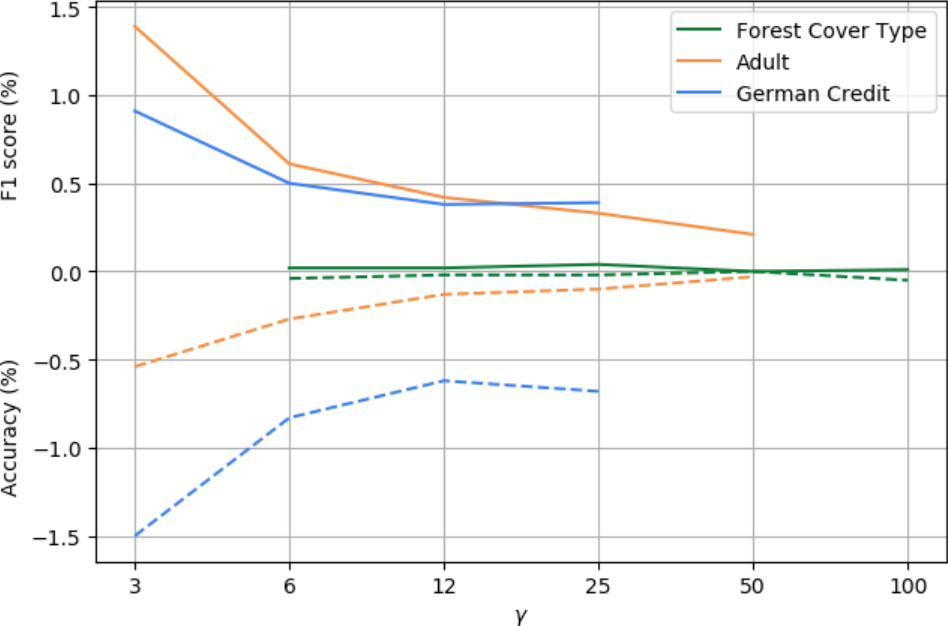
\includegraphics[width=0.8\textwidth]{Figures/classification-screenshot.PNG}
    \caption{Error in performance measures of the Random Forest classifier}
    \label{fig:classification-error}
\end{figure}

We obtain similar results with every other classifier, including Decision Tree, Logistic Regression, k-NN and Gradient Boosting. 
Our experiments with data fingerprinted with the second fingerprinting technique for categorical data based on finding the closest neighbourhood show very similar results to the naive approach. In future work, this technique will be more closely analysed, both from the robustness and the data utility point of view. In this case, the technique did not show distinctively better results than the naive approach. However, this might be case-specific and differ for the other choices of the parameter $k$ that defines the size of the neighbourhood. 
